
%(BEGIN_QUESTION)
% Copyright 2008, Tony R. Kuphaldt, released under the Creative Commons Attribution License (v 1.0)
% This means you may do almost anything with this work of mine, so long as you give me proper credit

A precision balance-beam scale is used in a doctor's office to weigh patients.  Weights are placed on the end of the beam until the beam returns to a balanced condition.  The number of weights placed on the beam becomes a reflection of the patient's weight:

$$\includegraphics[width=15.5cm]{i00466x01.eps}$$

However, the doctor is lazy.  He doesn't want to manually place the weights on the beam to weigh every patient any more.  Instead, he wants to have a gauge in his office to read out each patient's weight so he won't have to leave his chair.

\vskip 10pt

\noindent
Credit will be given for determining the following:

\begin{itemize}
\item{} Identify whether the basic scale mechanism is based on the {\it force-balance} principle or the {\it motion-balance} principle
\item{} Sketch the proper location to place a flapper/nozzle assembly
\item{} Sketch the proper location to place a feedback bellows
\item{} Sketch the correct pneumatic tube connections between a restrictor, the nozzle, the bellows, and the gauge in the doctor's office
\end{itemize}

Feel free to sketch your answers on this diagram (minus the weights and indicator):

\vskip 40pt

$$\includegraphics[width=15.5cm]{i00466x02.eps}$$

\underbar{file i00466}
%(END_QUESTION)





%(BEGIN_ANSWER)

(2 points): The scale works on the {\bf force-balance} principle

\vskip 10pt

This is but one possible solution -- there are others!

$$\includegraphics[width=15.5cm]{i00466x03.eps}$$

Credit 2 points for workable flapper/nozzle location, 2 points for workable feedback bellows, and 4 points for the rest (tubing, restrictor, gauge, supply)

%(END_ANSWER)





%(BEGIN_NOTES)

{\bf This question is intended for exams only and not worksheets!}.

%(END_NOTES)


